\documentclass{beamer}

\usepackage{comment}
\usepackage{color}
\usepackage{listings}
\usepackage{verbatim}
\usepackage{multicol}
\usepackage{booktabs}
\usepackage{textpos}
\usepackage{graphicx}
\usepackage{graphics}
\definecolor{green}{RGB}{0,128,0}

\newcommand\gehcomment[1]{{{\color{orange} #1}}}
\newcommand\add[1]{{{\color{blue} #1}}}
\newcommand\remove[1]{\sout{{\color{red} #1}}}
\newcommand\codecomment[1]{{{\color{green} #1}}}
\newcommand\redcomment[1]{{{\color{red} #1}}}
\newcommand\bluecomment[1]{{{\color{blue} #1}}}
\newcommand\greencomment[1]{{{\color{green} #1}}}
\newcommand\magentacomment[1]{{{\color{magenta} #1}}}

\begin{document}
\title{1D Hot Steam Injection\ldots}
\author{Michael Nole}
\date{\today}

%\frame{\titlepage}

%-----------------------------------------------------------------------------
\section{Description of Multiphase Regional Flow Scenario}

\subsection{Multiphase Regional Flow Conceptual Model}

\frame{\frametitle{Description of Multiphase Regional Flow Scenario}

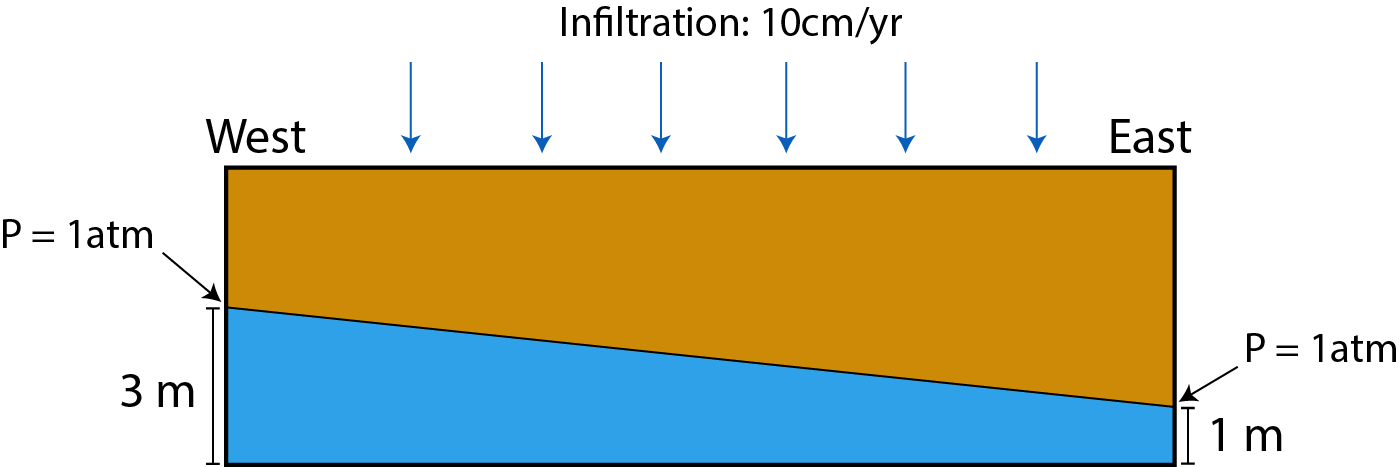
\includegraphics[height=1in]{./multiphase_regional_flow.png}

The ``Multiphase Regional Flow Scenario'' simulates an aquifer with a sloping water table and recharge using \redcomment{GENERAL MODE}. This scenario demonstrates how to make a gridded dataset to define boundary conditions and interpolate between them.

This demonstration follows several steps:

\begin{itemize}
  \small
  \item Simulate recharge at the West boundary in 1D until steady-state
  \item Simulate recharge at the East boundary in 1D until steady-state 
  \item Generate a gridded dataset with steady-state variables corresponding to GENERAL mode BC's and IC's
  \item Import the gridded dataset, interpolate within for IC's in 2D, and run to steady-state.
  \item Visualize in Paraview
\end{itemize}
}

%-----------------------------------------------------------------------------
\section{Description of Input Deck}

%-----------------------------------------------------------------------------
\subsection{DESCRIPTION}

\begin{frame}[fragile]\frametitle{DESCRIPTION}

The 1D simulations are similar to the ``1D Variably-Saturated Flow Scenario'':

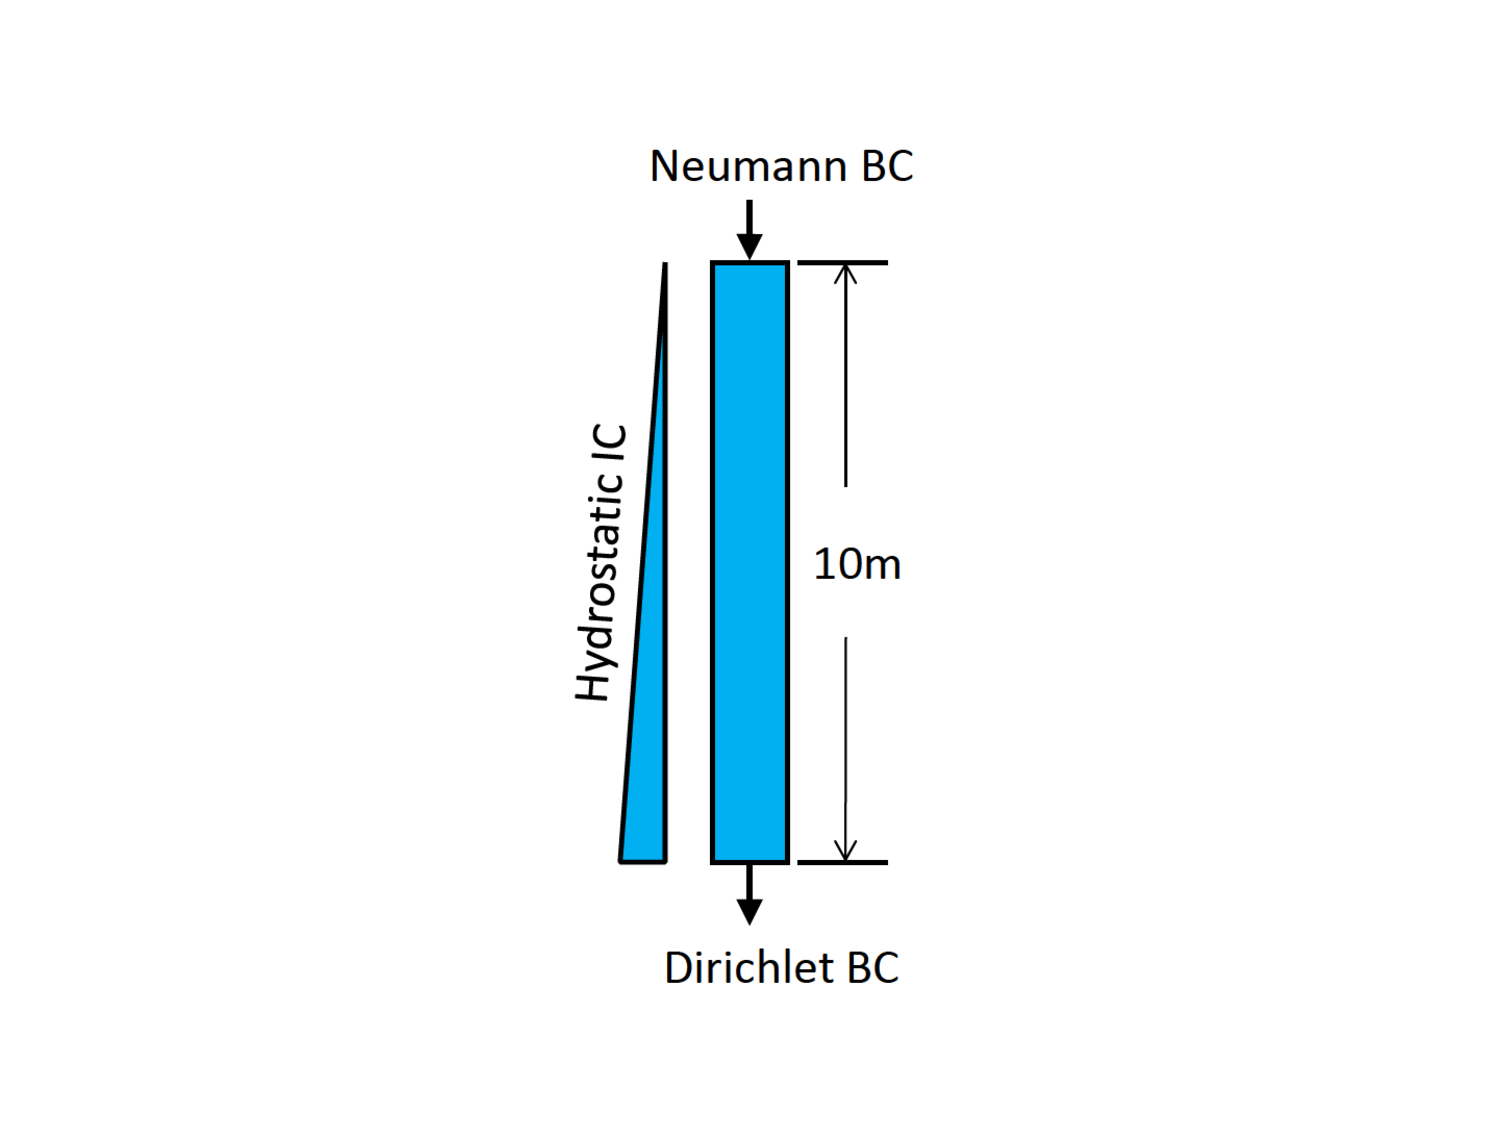
\includegraphics[height=3in]{../../1D_variably_saturated_flow/doc/vsat_flow_uniform.pdf}

\end{frame}

%-----------------------------------------------------------------------------
\subsection{SIMULATION\_WEST}

\begin{frame}[fragile]\frametitle{SIMULATION: West}

\begin{itemize}
\item Specify General flow mode
\end{itemize}


\begin{semiverbatim}

SIMULATION
  SIMULATION_TYPE SUBSURFACE
  PROCESS_MODELS
    SUBSURFACE_FLOW flow
      MODE GENERAL
      OPTIONS
        RESTRICT_STATE_CHANGE
        ANALYTICAL_JACOBIAN
        USE_INFINITY_NORM_CONVERGENCE
      /
    /
  /
END
\end{semiverbatim}

\end{frame}

%-----------------------------------------------------------------------------
\subsection{SOLVER}
\begin{frame}[fragile]\frametitle{SOLVER}

\begin{itemize}
  \item Specify direct solver (small problem)
\end{itemize}

\begin{semiverbatim}
LINEAR_SOLVER FLOW
  SOLVER DIRECT
END
\end{semiverbatim}
\end{frame}
%-----------------------------------------------------------------------------
\subsection{GRID}
\begin{frame}[fragile,containsverbatim]\frametitle{GRID}

\begin{itemize}
  \item Problem domain: $1 \times 1 \times 10$ m
  \item Grid resolution $1 \times 1 \times 0.1$ m
\end{itemize}

\begin{semiverbatim}
GRID
  TYPE STRUCTURED
  NXYZ 1 1 100
  BOUNDS
    0.d0 0.d0 0.d0
    1.d0 1.d0 10.d0
  /
END
\end{semiverbatim}

\end{frame}
%-----------------------------------------------------------------------------
\subsection{MATERIAL\_PROPERTY}

\begin{frame}[fragile,containsverbatim]\frametitle{MATERIAL\_PROPERTY}

\begin{semiverbatim}
MATERIAL_PROPERTY soil1
  ID 1
  CHARACTERISTIC_CURVES default
  POROSITY 0.25
  TORTUOSITY 1.0
  ROCK_DENSITY 2700.
  THERMAL_CONDUCTIVITY_DRY 1.1d0 W/m-C
  THERMAL_CONDUCTIVITY_WET 1.1d0 W/m-C
  HEAT_CAPACITY 0.01 J/kg-C
  PERMEABILITY
    PERM_ISO 1.d-12 
  /
END
\end{semiverbatim}

\end{frame}
%-----------------------------------------------------------------------------
\subsection{FLUID\_PROPERTIES}
\begin{frame}[fragile,containsverbatim,allowframebreaks]\frametitle{Fluid Properties}

\begin{itemize}
  \item Define properties of water and gas
  \begin{itemize}
    \item Diffusion coefficients
    \item Equations of state
  \end{itemize}
\end{itemize}

\begin{semiverbatim}
FLUID_PROPERTY
  PHASE LIQUID
  DIFFUSION_COEFFICIENT 1.d-9
END

FLUID_PROPERTY
  PHASE GAS
  DIFFUSION_COEFFICIENT 1.d-5
END

\newpage

EOS WATER
  DENSITY IF97
  ENTHALPY IF97
  STEAM_DENSITY IF97
  STEAM_ENTHALPY IF97
END

EOS GAS
  DENSITY DEFAULT
  VISCOSITY DEFAULT
  HENRYS_CONSTANT DEFAULT
END

\end{semiverbatim}

\end{frame}

%-----------------------------------------------------------------------------
\subsection{CHARACTERISTIC\_CURVES}

\begin{frame}[fragile,containsverbatim, allowframebreaks]\frametitle{CHARACTERISTIC\_CURVES}

\begin{itemize}
\item Set VG parameters
\end{itemize}

\begin{semiverbatim}
SATURATION_FUNCTION VAN_GENUCHTEN
    ALPHA 1.d-4
    M 0.5d0
    LIQUID_RESIDUAL_SATURATION 0.1d0
    CALCULATE_INTERFACIAL_TENSION
  /
\end{semiverbatim}

\newpage
\begin{itemize}
\item Burdine relative permeability
\end{itemize}

\begin{semiverbatim}
  PERMEABILITY_FUNCTION BURDINE_BC_LIQ
    PHASE LIQUID
    LAMBDA 2
    LIQUID_RESIDUAL_SATURATION 0.1d0
  /

  PERMEABILITY_FUNCTION BURDINE_BC_GAS
    PHASE GAS
    LAMBDA 2
    LIQUID_RESIDUAL_SATURATION 0.1d0
    GAS_RESIDUAL_SATURATION 0.1d0
  /
END
\end{semiverbatim}

\end{frame}

%-----------------------------------------------------------------------------
\subsection{OUTPUT}

\begin{frame}[fragile]\frametitle{OUTPUT}

\begin{semiverbatim}
OUTPUT
  TIMES y 0.01 0.1 1.0
  FORMAT TECPLOT POINT
  SNAPSHOT_FILE
    FORMAT HDF5 \bluecomment{! HDF5 file will be used to} 
    TIMES y 220.d0 \bluecomment{! set the 2D BC's}
  /
END
\end{semiverbatim}

\end{frame}

%-----------------------------------------------------------------------------
\subsection{TIME}

\begin{frame}[fragile]\frametitle{TIME}

\begin{itemize}
\item Run simulation to steady-state
\end{itemize}

\begin{semiverbatim}

TIME
  FINAL_TIME 220.d0 y
  INITIAL_TIMESTEP_SIZE 1.d0 h
  MAXIMUM_TIMESTEP_SIZE 5.d0 y
END

\end{semiverbatim}

\end{frame}

%-----------------------------------------------------------------------------
\subsection{REGION}

\begin{frame}[fragile,containsverbatim,allowframebreaks]\frametitle{REGION}

\begin{itemize}
  \item Delineate regions in the 1D domain for:
  \begin{itemize}
    \item top boundary face
    \item bottom boundary face
    \item entire domain (all)
  \end{itemize}
\end{itemize}

\begin{semiverbatim}
REGION all
  COORDINATES
    0.d0 0.d0 0.d0
    1.d0 1.d0 10.d0
  /
END

\newpage
REGION top
  FACE TOP
  COORDINATES
    0.d0 0.d0 10.d0
    1.d0 1.d0 10.d0
  /
END

REGION bottom
  FACE BOTTOM
  COORDINATES
    0.d0 0.d0 0.d0
    1.d0 1.d0 0.d0
  /
END
\end{semiverbatim}

\end{frame}

%-----------------------------------------------------------------------------
\subsection{FLOW\_CONDITION}

\begin{frame}[fragile,allowframebreaks]\frametitle{FLOW\_CONDITION}

\begin{itemize}
\item Initially partially-saturated (at residual liquid saturation)
\item Constant pressure and temperature BC's, water table is at 3m
\end{itemize}

\begin{semiverbatim}
FLOW_CONDITION liquid_pressure
  TYPE
    LIQUID_PRESSURE HYDROSTATIC
    MOLE_FRACTION DIRICHLET
    TEMPERATURE DIRICHLET
  /
  DATUM 0.d0 0.d0 3.d0 \bluecomment{! Water table at 3m}
  LIQUID_PRESSURE 101325.d0
  MOLE_FRACTION 1.d-8
  TEMPERATURE 28.d0
END

\newpage
FLOW_CONDITION partially_saturated
  TYPE
    GAS_PRESSURE DIRICHLET
    GAS_SATURATION DIRICHLET
    TEMPERATURE DIRICHLET
  /
  GAS_PRESSURE 101256.d0
  GAS_SATURATION 8.9d-1 
  TEMPERATURE 25.d0

END

\newpage
FLOW_CONDITION unsaturated
  TYPE
    GAS_PRESSURE DIRICHLET
    RELATIVE_HUMIDITY DIRICHLET
    TEMPERATURE DIRICHLET
  /
  GAS_PRESSURE 101256.d0
  RELATIVE_HUMIDITY 0.5
  TEMPERATURE 25.d0

END

FLOW_CONDITION recharge
  TYPE
    LIQUID_FLUX NEUMANN
    GAS_FLUX NEUMANN
    TEMPERATURE DIRICHLET
  /
  LIQUID_FLUX 10.d0 cm/y \bluecomment{! Infiltration occuring}
  GAS_FLUX 0.d0 cm/y     \bluecomment{! at 10cm/yr}
  TEMPERATURE 25.d0
END

\end{semiverbatim}

\end{frame}

%-----------------------------------------------------------------------------
\subsection{INITIAL\_CONDITION}

\begin{frame}[fragile]\frametitle{INITIAL\_CONDITION}

\begin{semiverbatim}
INITIAL_CONDITION
  FLOW_CONDITION partially_saturated 
  REGION all
END
\end{semiverbatim}

\end{frame}

%-----------------------------------------------------------------------------
\subsection{BOUNDARY\_CONDITION}

\begin{frame}[fragile]\frametitle{BOUNDARY\_CONDITION}

\begin{itemize}
\item Couple the \greencomment{left} and \greencomment{right} flow conditions with their corresponding regions.
\end{itemize}

\begin{semiverbatim}
BOUNDARY_CONDITION outlet
  FLOW_CONDITION liquid_pressure
  REGION bottom
END

BOUNDARY_CONDITION inlet
  FLOW_CONDITION recharge
  REGION top
END

BOUNDARY_CONDITION inlet
  FLOW_CONDITION unsaturated
  REGION top
END
\end{semiverbatim}

\end{frame}

%-----------------------------------------------------------------------------

\subsection{STRATA}

\begin{frame}[fragile]\frametitle{STRATA}

\begin{semiverbatim}

STRATA
  REGION all
  MATERIAL soil1
END

\end{semiverbatim}

\end{frame}

%-----------------------------------------------------------------------------
\subsection{west.in}

\begin{frame}[fragile]\frametitle{Running PFLOTRAN}

\begin{semiverbatim}

> cd $PFLOTRAN_DIR
> cd shortcourse/exercises/multiphase_regional_flow
> pflotran -input_prefix west
> python west.py &
\end{semiverbatim}

\end{frame}

%-----------------------------------------------------------------------------
\subsection{SIMULATION\_EAST}

\begin{frame}[fragile]\frametitle{SIMULATION: East}

\begin{semiverbatim}
FLOW_CONDITION liquid_pressure
  TYPE
    LIQUID_PRESSURE HYDROSTATIC
    MOLE_FRACTION DIRICHLET
    TEMPERATURE DIRICHLET
  /
  DATUM 0.d0 0.d0 1.d0  \bluecomment{! Water table is lower at the}
  LIQUID_PRESSURE 101325.d0 \bluecomment{! East boundary}
  MOLE_FRACTION 1.d-8
  TEMPERATURE 28.d0
END
\end{semiverbatim}

\end{frame}
%-----------------------------------------------------------------------------
\subsection{east.in}

\begin{frame}[fragile]\frametitle{Running PFLOTRAN}

\begin{semiverbatim}

> cd $PFLOTRAN_DIR
> cd shortcourse/exercises/multiphase_regional_flow
> pflotran -input_prefix east
> python east.py &
\end{semiverbatim}

\end{frame}

%-----------------------------------------------------------------------------
\subsection{make_gridded_dataset}

\begin{frame}[fragile]\frametitle{Make Gridded Dataset}

\begin{itemize}
\item From the east and west steady-state solutions, we will make a gridded dataset.
\end{itemize}

\begin{semiverbatim}
> cd $PFLOTRAN_DIR
> cd shortcourse/exercises/multiphase_regional_flow
> python make_dataset.py
\end{semiverbatim}

\begin{itemize}
\item Open ic\_dataset.h5 in HDF5View.
\end{itemize}

\end{frame}

%-----------------------------------------------------------------------------
\subsection{make_gridded_dataset}

\begin{frame}[fragile, allowframebreaks]\frametitle{DATASET: Multiphase Regional Flow}

\begin{itemize}
\item Setup 2D input deck: multiphase\_regional\_flow.in
\item Import newly-created dataset
\end{itemize}

\begin{semiverbatim}

DATASET liquid_pressure
  FILENAME ./ic_dataset.h5
  HDF5_DATASET_NAME bounding_liquid_pressure
END

DATASET mole_fraction
  FILENAME ./ic_dataset.h5
  HDF5_DATASET_NAME bounding_mole_fraction
END

\newpage

DATASET gas_pressure
  FILENAME ./ic_dataset.h5
  HDF5_DATASET_NAME bounding_gas_pressure
END

DATASET gas_saturation
  FILENAME ./ic_dataset.h5
  HDF5_DATASET_NAME bounding_gas_saturation
END

DATASET temperature
  FILENAME ./ic_dataset.h5
  HDF5_DATASET_NAME bounding_temperature
END

\end{semiverbatim}

\end{frame}
%-----------------------------------------------------------------------------
\subsection{Discretization}

\begin{frame}[fragile, allowframebreaks]\frametitle{GRID}

\begin{semiverbatim}
GRID
  TYPE STRUCTURED
  NXYZ 10 1 100
  BOUNDS
    0.d0 0.d0 0.d0
    100.d0 1.d0 10.d0
  /
END
\end{semiverbatim}

\end{frame}
%-----------------------------------------------------------------------------
\subsection{output}

\begin{frame}[fragile, allowframebreaks]\frametitle{OUTPUT}

\begin{semiverbatim}
OUTPUT
  SNAPSHOT_FILE
    FORMAT HDF5
    PERIODIC TIME 10. d between 0. y and 1. y
    PERIODIC TIME 100. d between 1. y and 2. y
    PERIODIC TIME 365. d between 2. y and 20. y
  /
END
\end{semiverbatim}

\end{frame}

%-----------------------------------------------------------------------------
\subsection{time}

\begin{frame}[fragile, allowframebreaks]\frametitle{TIME}

\begin{semiverbatim}
TIME
  FINAL_TIME 20.d0 y
  INITIAL_TIMESTEP_SIZE 1.d0 h
  MAXIMUM_TIMESTEP_SIZE 1.d0 y
END
\end{semiverbatim}

\end{frame}
%-----------------------------------------------------------------------------
\subsection{regions}

\begin{frame}[fragile, allowframebreaks]\frametitle{REGION}

\begin{semiverbatim}
REGION all
  COORDINATES
    0.d0 0.d0 0.d0
    100.d0 1.d0 10.d0
  /
END

REGION top
  FACE TOP
  COORDINATES
    0.d0 0.d0 10.d0
    100.d0 1.d0 10.d0
  /
END

\newpage
REGION bottom
  FACE BOTTOM
  COORDINATES
    0.d0 0.d0 0.d0
    100.d0 1.d0 0.d0
  /
END

REGION east
  FACE EAST
  COORDINATES
    100.d0 0.d0 0.d0
    100.d0 0.d0 10.d0
  /
END
\newpage
REGION west
  FACE WEST
  COORDINATES
    0.d0 0.d0 0.d0
    0.d0 0.d0 10.d0
  /
END
\end{semiverbatim}

\end{frame}
%-----------------------------------------------------------------------------
\subsection{flow\_conditions}

\begin{frame}[fragile, allowframebreaks]\frametitle{FLOW CONDITION}

\begin{semiverbatim}
FLOW_CONDITION initial
  TYPE
    LIQUID_PRESSURE DIRICHLET
    MOLE_FRACTION DIRICHLET
    TEMPERATURE DIRICHLET
    GAS_PRESSURE DIRICHLET
    GAS_SATURATION DIRICHLET
  / \bluecomment{! Here we use datasets to set initial conditions. PFLOTRAN} 
    \bluecomment{! interpolates between values automatically.}
  LIQUID_PRESSURE DATASET liquid_pressure 
  MOLE_FRACTION DATASET mole_fraction
  TEMPERATURE DATASET temperature
  GAS_PRESSURE DATASET gas_pressure
  GAS_SATURATION DATASET gas_saturation
END



FLOW_CONDITION unsaturated
  TYPE
    GAS_PRESSURE DIRICHLET
    #GAS_SATURATION DIRICHLET
    RELATIVE_HUMIDITY DIRICHLET
    TEMPERATURE DIRICHLET
  /
  GAS_PRESSURE DATASET gas_pressure 
  RELATIVE_HUMIDITY 0.5
  #GAS_SATURATION 8.9d-1 
  TEMPERATURE DATASET temperature 

END
\newpage
FLOW_CONDITION recharge
  TYPE
    LIQUID_FLUX NEUMANN
    GAS_FLUX NEUMANN
    TEMPERATURE DIRICHLET
  /
  LIQUID_FLUX 10.d0 cm/y 
  GAS_FLUX 0.d0 cm/y
  TEMPERATURE 25.d0
END
\end{semiverbatim}

\end{frame}
%-----------------------------------------------------------------------------
\subsection{boundary_conditions}

\begin{frame}[fragile, allowframebreaks]\frametitle{INITIAL and BOUNDARY CONDITION}

\begin{semiverbatim}
INITIAL_CONDITION
  FLOW_CONDITION initial
  REGION all
END

BOUNDARY_CONDITION bottom
  FLOW_CONDITION initial
  REGION bottom
END

BOUNDARY_CONDITION top
  FLOW_CONDITION recharge
  REGION top
END
\newpage
BOUNDARY_CONDITION top
  FLOW_CONDITION unsaturated
  REGION top
END

BOUNDARY_CONDITION east
  FLOW_CONDITION initial
  REGION east
END

BOUNDARY_CONDITION west
  FLOW_CONDITION initial
  REGION west
END
\end{semiverbatim}

\end{frame}

%-----------------------------------------------------------------------------
\subsection{multiphase_regional_flow.in}

\begin{frame}[fragile]\frametitle{Running PFLOTRAN}

\begin{semiverbatim}

> cd $PFLOTRAN_DIR
> cd shortcourse/exercises/multiphase_regional_flow
> pflotran -input_prefix multiphase_regional_flow
\end{semiverbatim}

\end{frame}

%-----------------------------------------------------------------------------
\subsection{visualize_in_paraview}

\begin{frame}[fragile]\frametitle{Visualize in Paraview}

\begin{itemize}
\item In Paraview, load "multiphase\_regional\_flow.h5" as a PFLOTRAN file
\item Re-orient (+Y) and apply all variables.
\item Filters --  Annotation -- Annotate Time Filter
\item Select Liquid Saturation
\item Play
\end{itemize}

\end{frame}

\end{document}
